\documentclass[aspectratio=169]{beamer}
\usepackage[utf8]{inputenc}

% design
\usetheme{CambridgeUS}
\usecolortheme{beaver}
\setbeamertemplate{itemize items}[square]
\usenavigationsymbolstemplate{\beamertemplatenavigationsymbolsempty}
\definecolor{darkred}{rgb}{0.8,0,0}
\colorlet{grey1}{gray!10!white} % I think = RGB 0.95 0.95 0.95
\colorlet{grey2}{gray!60!white} % I think = RGB 0.7 0.7 0.7
\setbeamercolor{structure}{fg=darkred}
\setbeamertemplate{enumerate item}{\insertenumlabel.}
\setbeamertemplate{itemize item}{$\blacktriangleright$}
\setlength{\tabcolsep}{12pt}
\setbeamercolor{block title}{fg=darkred}

% bibliography
%\usepackage[backend=biber, style=authortitle]{biblatex}
\usepackage{natbib}
\usepackage{har2nat}
\bibliographystyle{unsrt}
%\addbibresource{../../smc.bib}
\usepackage{bibentry}
\nobibliography*

% tikz
\usepackage{tikz}
\usetikzlibrary{positioning}

% maths
\usepackage{amsmath}
\usepackage{amssymb}
\usepackage{amsfonts}
\usepackage{amsthm}
\theoremstyle{definition}
\newtheorem{defn}{Definition}

% useful math symbols
\newcommand{\PR}{\mathbb{P}}
\newcommand{\E}{\mathbb{E}}
\newcommand{\V}{\operatorname{Var}}
\newcommand{\eqdist}{\overset{d}{=}}
\newcommand{\I}[1]{\mathbb{I}\{#1\}}
\newcommand{\Ntoinfty}{\overset{N\to\infty}{\longrightarrow}}
\newcommand{\limNtoinfty}{\underset{N\to\infty}{\lim}}
\newcommand\indep{\protect\mathpalette{\protect\independenT}{\perp}}
\def\independenT#1#2{\mathrel{\rlap{$#1#2$}\mkern2mu{#1#2}}}

% distributions
\newcommand{\N}{\mathcal{N}}
\newcommand{\Cat}{\operatorname{Categorical}}
\newcommand{\Unif}{\operatorname{Uniform}}
\newcommand{\Mn}{\operatorname{Multinomial}}
\newcommand{\Bin}{\operatorname{Binomial}}

% project-specific commands
\newcommand{\F}{\mathcal{F}_{t-1}}
\newcommand{\vt}[2][t]{\nu_{#1}^{(#2)}}
%\newcommand{\vt}[1]{v_{#1}}
\newcommand{\wt}[2][t]{w_{#1}^{(#2)}}
%\newcommand{\wt}[1]{w_{#1}}
%\newcommand{\wbar}[2][t]{\bar{w}_{#1}^{(#2)}}
%\newcommand{\vttilde}[2][t]{\tilde{v}_{#1}^{(#2)}}
\newcommand{\Et}{\mathbb{E}_{t}}

\title[]{Asymptotic genealogies of non-neutral populations}
\author[Suzie Brown]{\textbf{Suzie Brown} \\[5pt] University of Warwick, U.K. \\ with Paul Jenkins, Adam Johansen \& Jere Koskela}
\date{13 May 2021} 

\begin{document}
\begin{frame}
\maketitle
\end{frame}


\begin{frame}{Interacting particle system}
?
\end{frame}


\begin{frame}{Kingman's $n$-coalescent}%\footnote[frame]{Kingman 1982}}
\begin{columns}
\begin{column}{0.45\textwidth}
\begin{itemize}
\item Continuous-time Markov chain on the space of partitions of $\{1,\dots,n\}$
\item Single pair mergers only
\item Each pair merges independently at rate 1 (total merge rate $\binom{k}{2}$ while there are $k$ distinct lineages)
\end{itemize}
\end{column}
\begin{column}{0.45\textwidth}
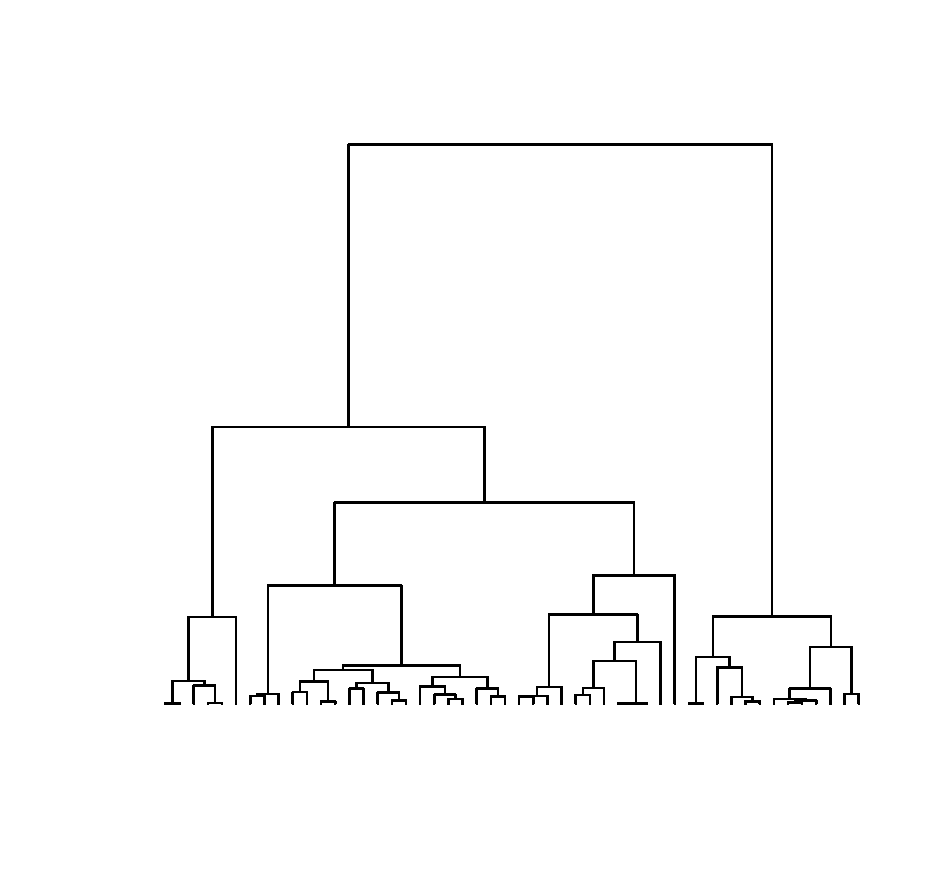
\includegraphics[width=\textwidth, trim={2.8cm 3cm 1.5cm 2cm}, clip]{ncoalescent.pdf}
\end{column}
\end{columns}
\end{frame}


\begin{frame}{Scenario}
\begin{itemize}
\item Fixed population size $N$
\item Discrete generations
\item Sample $n \leq N$ individuals from the terminal generation
\item Rescale to continuous time
\item Let $N\to\infty$
\end{itemize}
\end{frame}


\begin{frame}{Sufficient conditions, neutral models}
\begin{theorem}[Kingman 1982]
\begin{itemize}
\item Individuals are exchangeable
\item Offspring counts $\nu^{(1:N)}$ are i.i.d. across generations
\item $\V[ \nu^{(1)} ] = \sigma_N^2 \longrightarrow \sigma^2 \in (0,\infty)$
\item $\sup_N \E[ (\nu^{(1)})^k] <\infty$ for all $k\geq 3$
\end{itemize}
Then the rescaled genealogy of $n$ individuals converges weakly to the $n$-coalescent as $N\to\infty$.
\end{theorem}
\end{frame}


\begin{frame}{Sufficient conditions, neutral models}
\begin{itemize}
\item Exchangeability = neutrality (genotype does not affect number of offspring)
\item Since $\sum \nu^{(i)} = N$ and individuals are exchangeable, $\E[\nu^{(i)}] = 1$.
\item Case $\sigma^2 = 0$ would mean no coalescences in the limit
\item Conditions can be verified for e.g.\ Moran \& Wright-Fisher models
\end{itemize}
\end{frame}


\begin{frame}{Necessary and sufficient conditions, neutral models}
\begin{theorem}[M\"ohle Sagitov 2001, 2003]
\begin{itemize}
\item Individuals are exchangeable
\item Offspring counts $\nu^{(1:N)}$ are i.i.d. across generations
\item $c_N >0$ for all $N<\infty$
\item $c_N \longrightarrow 0$
\item $d_N/c_N \longrightarrow 0$
\end{itemize}
If and only if the rescaled genealogy of $n$ individuals converges weakly to the $n$-coalescent as $N\to\infty$.
\end{theorem}
\begin{equation*}
d_N := \frac{N \E[ ( \nu^{(1)} )_3 ] }{(N)_3}  ,\qquad
c_N := \frac{N \E[ ( \nu^{(1)} )_2 ] }{(N)_2} 
\end{equation*}
\end{frame}


\begin{frame}{Necessary and sufficient conditions, neutral models}
\begin{itemize}
\item The condition $c_N >0$ plays the same role as Kingman's condition $\sigma^2 >0$
\item $c_N = \frac{\V[\nu^{(1)}]}{N-1}$, so $c_N \to 0$ is less restrictive than Kingman's condition $\V[ \nu^{(1)} ] \to \sigma^2$
\item Only requires control up to 3rd moment, cf.\ Kingman requires \emph{all} moments finite
\end{itemize}
\end{frame}


\begin{frame}{Sufficient conditions, non-neutral models}
\begin{theorem}[B Koskela Jenkins Johansen 2021]
\begin{itemize}
\item Given $\nu_t^{(1:N)}$, assignment of offspring to parents is uniform over all valid assignments
\item Time scale is almost surely finite
\item $\exists$ deterministic sequence $b_N \to 0$ such that $\forall N, t$
\begin{equation*}
\frac{1}{(N)_3} \sum_{i=1}^N \E_t[ (\nu_t^{(i)})_3 ]
\leq b_N \frac{1}{(N)_2} \sum_{i=1}^N \E_t[ (\nu_t^{(i)})_2 ]
\end{equation*}
\end{itemize}
Then the rescaled genealogy of $n$ individuals converges weakly to the $n$-coalescent as $N\to\infty$.
\end{theorem}
\end{frame}


\begin{frame}{Sufficient conditions, non-neutral models}
\begin{itemize}
\item Not exchangeable, so individual index kept explicit
\item Not i.i.d. over time, so $t$ kept explicit, and time scale is not constant!
\item The finite time scale condition plays the same role as Kingman's $\sigma^2>0$ 
\item The main condition is the non-exchangeable analogue of M\"ohle \& Sagitov's $d_N/c_N \to 0$
\end{itemize}
\end{frame}


\begin{frame}{In conclusion...}
\begin{itemize}
\item ?
\end{itemize}
\end{frame}


\begin{frame}{References}
\begin{enumerate}
\item JFC Kingman (1982) \textit{The coalescent}. Stochastic Processes and Their Applications 13:235--248.
\item JFC Kingman (1982) \textit{On the genealogy of large populations}. Journal of Applied Probability 19A:27--43.
\item M M\"ohle, S Sagitov (2001) \textit{A classification of coalescent processes for haploid exchangeable population models}. The Annals of Probability 29(4):1547--1562.
\item M M\"ohle, S Sagitov (2003) \textit{Coalescent patterns in diploid exchangeable population models}. Journal of Mathematical Biology 47(4):337--352.
\item S Brown, PA Jenkins, AM Johansen, J Koskela (2021) \textit{Simple conditions for convergence of sequential Monte Carlo genealogies with applications}. Electronic Journal of Probability 26:1--22.
\end{enumerate}
\end{frame}

\end{document}